\documentclass[a4paper,12pt]{article}
\usepackage[a4paper,top=3cm,bottom=2cm,left=3cm,right=3cm,marginparwidth=1.75cm]{geometry}
\usepackage[brazil]{babel}
\usepackage[T1]{fontenc}
\usepackage[utf8]{inputenc}
\usepackage{amsmath}
\usepackage{MnSymbol}
\usepackage{wasysym}
\usepackage{hyperref}
\usepackage{color}
\definecolor{Blue}{rgb}{0,0,0.9}
\definecolor{Red}{rgb}{0.9,0,0}
\usepackage{esvect}
\usepackage{graphicx}
\usepackage{float}
\usepackage{indentfirst}
\usepackage{caption}
\usepackage{blkarray}
\newcommand\Mark[1]{\textsuperscript#1}
\usepackage{pgfplots}
\usepackage{amsfonts}
\title{Relatório de Laboratório 2}
\author{Guilherme Philippi, Carlos Eduardo dos Santos Junior}
\begin{document}
\maketitle
\tableofcontents

\section{Grafos: Aspectos Gerais\label{sec:grafos}}
Esta seção tem como objetivo apresentar um breve resumo da \textit{teoria de grafos}, tema muito estudado por diversos matemáticos e aplicado em diversas áreas do conhecimento para além da matemática.

Podemos dizer que em 1736 é que a teoria teve início, com base no artigo publicado por Leonhard Euler, sobre as 7 pontes de Königsberg \cite{euler:KOENIGSBERG} \cite{grafos1}. Esse é o problema que normalmente introduz quem está começando a trabalhar com grafos --- se trata do desafio de ligar todos os pontos de um desenho sem tirar o lápis do papel e sem passar duas vezes no mesmo ponto. Segundo a história, os moradores daquela região perguntavam se era possível atravessar todas as pontes sem ter que repetir alguma delas. Euler provou que isso não era possível, ao formular matematicamente o problema, que deu origem a esta teoria.

Para isso, Euler abstraiu o problema, ao vê-lo de um ponto de vista matemático, como um conjunto de pontos intersectados por linhas (vide Figura ~\ref{fig:koni}). Essa representação facilitou a análise de que a solução do problema só seria possível se houvesse exatamente zero ou dois pontos de onde saísse um número ímpar de caminhos \cite{euler:KOENIGSBERG}.

\begin{figure}[H]
	\begin{center}
		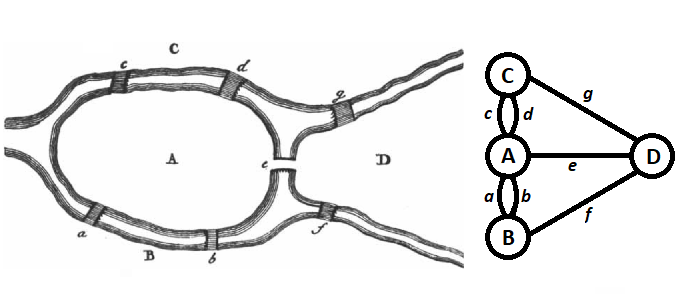
\includegraphics[width=0.85\linewidth]{koenigsbern.png}
	\end{center}
	\caption{Ilustração original do problema \cite{euler:KOENIGSBERG} e sua representação em Grafos.}
	\label{fig:koni}
\end{figure}

Além dessa, muitas outras situações reais podem ser convenientemente representadas por simples diagramas contendo um conjunto de pontos e linhas ligando pares desses pontos. Por exemplo, podemos definir o conjunto $P = \{a,b,c\}$ das pessoas $a, b$ e $c$ e um conjunto $A = \{\{a,b\}, \{b,c\}\}$ como o conjunto de amizades entre essas pessoas --- no caso, $a$ é amigo de $b$, que é amigo de $c$, porém $a$ não é amigo de $c$. 

\begin{center}
	\begin{minipage}{0.9 \linewidth}
		\textbf{Grafo:} Um grafo $G$ é uma tripla ordenada da forma $(V(G),E(G), \psi_{G})$, composto por um conjunto de \textit{vértices} $V(G)$, de arestas $E(G)$ e uma \textit{função de incidência} $\psi_{G}$ que, por sua vez, associa a cada aresta de $V(G)$ um par não ordenado de vértices (nem sempre distintos) de $E(G)$. Costumamos dizer que as arestas ligam os vértices.
	\end{minipage}
\end{center}

Existe, também, uma íntima relação entre Grafos e algoritmos. De fato, podemos inclusive representar um algoritmo por um grafo \cite{grafos0}. Na verdade, a definição de grafos é tão abrangente que podemos ver suas ligações com diversas áreas do conhecimento. 

No que se segue, definiremos algumas características elementares que serão utilizadas durante esse texto. Para um estudo mais completo sobre essa teoria, vide \cite{grafos1} e \cite{grafosPremioElon}.

\subsection{Algumas Classificações Importantes}

Existem duas definições de extrema importância para o nosso problema molecular (tema central desse texto): o conceito de grafo completo e o de estruturas $k$-cliques. Porém, seremos obrigado a definir alguns outros conceitos prévios, como segue. 


\begin{center}
	\begin{minipage}{0.9 \linewidth}
		\textbf{Laço:} Uma aresta $\{e_i, e_j\} \in E$ tal que $i = j$.
	\end{minipage}
\end{center}

Também, caso existam duas arestas iguais ($\{e_i, e_j\}$ e 
$\{e_j, e_i\}$, por exemplo, lembrando que $E$ é um conjunto de pares não ordenados), com as mesmas extremidades, estas recebem o nome de \textbf{arestas paralelas}.

\begin{center}
	\begin{minipage}{0.9 \linewidth}
		\textbf{Grafo simples}: Um grafo que não possui laços ou arestas paralelas.
	\end{minipage}
\end{center}

\begin{center}
	\begin{minipage}{0.9 \linewidth}
		\textbf{Grafo Completo:} É um grafo simples em que todo vértice é conectado a todos os outros vértices.
	\end{minipage}
\end{center}

\begin{figure}[H]
	\begin{center}
		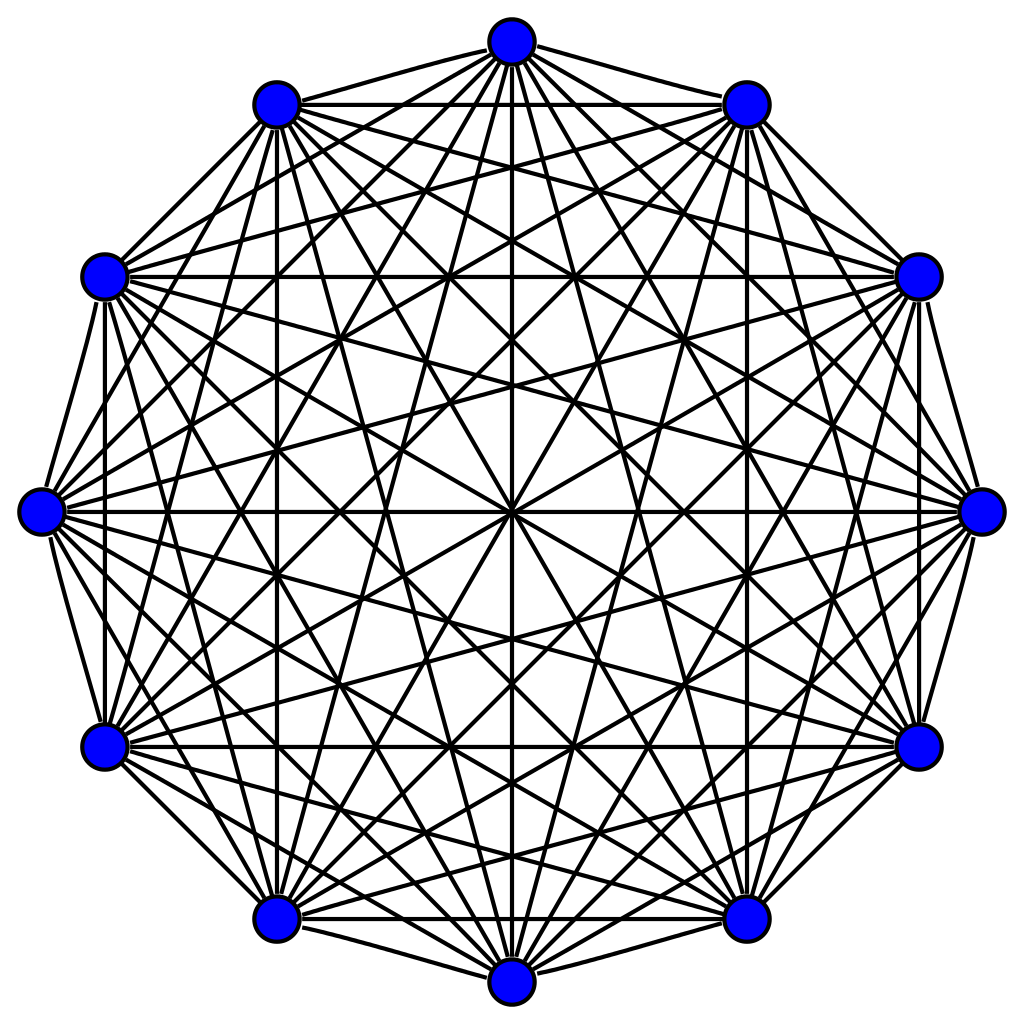
\includegraphics[width=0.4\linewidth]{grafocompleto.png}
	\end{center}
	\caption{Diagrama de um grafo completo com 12 vértices ($|V| = 12$).}
	\label{fig:grafocompleto}
\end{figure}

Outro conceito que nos será de grande utilidade é o de subgrafo.
\begin{center}
	\begin{minipage}{0.9 \linewidth}
		\textbf{Subgrafo:} É um grafo resultante de um subconjunto de vértices e outro subconjunto de arestas de outro grafo. Isto é, seja $G = (V, E), G^\prime = (V^\prime, E^\prime)$ é dito um subgrafo de $G$ se $(V^\prime, E^\prime)$ é um grafo tal que $V^\prime \subseteq V$ e $E^\prime \subseteq E$.
	\end{minipage}
\end{center}

E, finalmente
\begin{center}
	\begin{minipage}{0.9 \linewidth}
		\textbf{$k$-Clique}: é um subgrafo $G^\prime$ com $k$ vértices tal que $G^\prime$ é completo.
	\end{minipage}
\end{center}

Em especial, também podemos interpretar as arestas como \textit{caminhos} e, se o fizermos, podemos pensar em alguma forma de métrica para esses caminhos. Esse pensamento da origem à nossa última definição de grafos, ditos \textit{ponderados}.

\begin{center}
	\begin{minipage}{0.9 \linewidth}
		\textbf{Grafo Ponderado:} É um grafo que possui uma função $d(E) \rightarrow \mathbb{R}$ associada, isto é, o grafo que possui valores numéricos atribuídos as suas arestas.
	\end{minipage}
\end{center}

\phantomsection
\addcontentsline{toc}{section}{Referências}

\bibliographystyle{unsrt}
\bibliography{references}

\end{document}
